\documentclass{article}

\setlength{\parindent}{0em}
\setlength{\parskip}{0.8em}
\linespread{1.05}

\usepackage{amsmath}
\usepackage{algorithm}
\usepackage[noend]{algpseudocode}
\usepackage{booktabs}
\usepackage[usenames, dvipsnames]{color}
\usepackage{colortbl}
\usepackage[shortlabels]{enumitem}
\usepackage{extarrows}
\usepackage{fancyhdr}
\usepackage[T1]{fontenc}
\usepackage[left = 1in, right = 1in, top = 1in, bottom = 1in]{geometry}
\usepackage{graphicx}
\usepackage{hyperref}
\usepackage{lastpage}
\usepackage{listings}
\usepackage{mathpazo}
\usepackage{mathtools}
\usepackage{pdfpages}
\usepackage[protrusion = true, expansion = true]{microtype}
\usepackage{multirow}
\usepackage{subfigure}
\usepackage{wrapfig}
\usepackage{xcolor}

\hypersetup{colorlinks = true, urlcolor = blue}

\definecolor{DarkGreen}{rgb}{0.0,0.4,0.0}
\definecolor{highlight}{RGB}{255,251,204}

\lstdefinestyle{Style1}{
	backgroundcolor = \color{highlight},
	basicstyle = \footnotesize\ttfamily,
	breakatwhitespace = false,
	breaklines = true,
	captionpos = b,
	commentstyle = \usefont{T1}{pcr}{m}{sl}\color{DarkGreen},
	deletekeywords = {},
	escapeinside = {\%},
	firstnumber = 1,
	frame = single,
	% frameround = tttt,
	keywordstyle = \color{Blue}\bf,
	language = Perl,
	morekeywords = {},
	numbers = left,
	numbersep = 10pt,
	numberstyle = \tiny\color{Gray},
	rulecolor = \color{black},
	showstringspaces = false,
	showtabs = false,
	stepnumber = 5,
	stringstyle = \color{Purple},
	tabsize = 2,
}

\newcommand{\insertcode}[2]{
	\begin{itemize}
		\item[]
			\lstinputlisting[caption = #2, label = #1, style = Style1]{#1}
	\end{itemize}}

\newenvironment{innerlist}[1][\enskip\textbullet]{
	\begin{itemize}[
			#1, leftmargin = 2em, parsep = 0pt, itemsep = 0pt, topsep = 0pt, partopsep = 0pt
			]
		}{\end{itemize}}

\pagestyle{fancy}
\lhead{}
\chead{}
\rhead{}
\cfoot{{\arabic{page} / \protect\pageref{LastPage}}}
\renewcommand{\headrulewidth}{0pt}

\makeatletter
\renewcommand{\@listI}{\itemsep=0pt}

\renewcommand{\maketitle}{
	\begin{flushright}
		{\LARGE\@title}

		\vspace{50pt}

		{\large\@author}
		\\\@date

		\vspace{30pt}
	\end{flushright}
}

\title{\textbf{Introduction to Database Systems} \\
	Efficient Sub-sequence Matching in Time Series Using a Cluster}

\author{\textsc{Hengbin Liao, Jun Xu}
	\\{Boston University}}

\date{\today}

\begin{document}
\maketitle

\section{Introduction}
A time series is a sequence of data points, typically consisting of successive measurements made over a time interval. Examples of time series are ocean tides, counts of sunspots, and the daily closing value of the Dow Jones Industrial Average. Time series are used in statistics, signal processing, pattern recognition, econometrics, mathematical finance, weather forecasting, and largely in any domain of applied science and engineering which involves temporal measurements. \par

Given a query time series and a database of time series, subsequence matching of time series is the problem of identifying the database subsequence (i.e., some part of some time series in the database) that is the most similar to the query sequence. It's important for subsequence matching to be efficient in domains where the database sequences are much longer than the queries.

\section{Using Embedding for Subsequence Matching}
Given $X = (X_1, \cdots, X_{|X|})$, a database sequence that is relative long, containing for example millions of elements, we can concatenate all $X_j, \forall j = 1, \cdots, |X|$. Called it $X$, too. \par

Also given a query sequence $Q$, we want to find the subsequence of $X$ that optimally matches $Q$ under Dynamic Time Warping. Brute-force search will be too expensive to afford. We cited the method called \emph{Approximate Embedding-based Subsequence Matching of Time Series}. This method maps every query $Q$ into a $d$-dimensional vector and every element $X_j$ of the database sequence also into a $d$-dimensional vector. \par

Define \emph{reference sequence} $R$ as a relative short sequence. Then the 1D embedding for the database sequence $$F^R(X, j) = D_{|R|,j}(R, X),$$ i.e., the smallest possible cost of matching $(R_1, \cdots, R_{|R|})$ to any suffix of $(X_1, \cdots, X_j)$. And the 1D embedding for the query is $$F^R(Q) = D_{|R|,|Q|}(R, Q),$$ i.e., the smallest possible cost of matching $(R_1, \cdots, R_{|R|})$ to any suffix of $(Q_1, \cdots, Q_{|Q|})$. If we pick multiple reference sequences to create a multidimensional embedding, we can define a $d$-dimensional embedding $F$ as follows: 
$$F(X,j) = (F^{R_1}(X,j), \cdots, F^{R_d}(X,j)).$$
$$F(Q) = (F^{R_1}(Q), \cdots, F^{R_d}(Q)).$$
Computing such a vector for the database sequence is an off-line preprocessing step that takes time in $O(|X|\sum_{i=1}^d|R_i|)$. And for a query $Q$, its embedding vector is computed online, by applying the DTW algorithm $d$ times, with inputs $R_i$ and $Q$. In total, this applications of DTW take time in $O(|Q|\sum_{i=1}^d|R_i|)$. This time is negligible compared to running the DTW algorithm between $Q$ and $X$, which takes $O(|Q||X|)$ time. \par

Therefore, rather than brute force search, we do as follows:
\begin{innerlist}
\item Compare $F(Q)$ to $F(X,j),\ \forall j=1,\cdots,|X|$.
\item Choose $j$'s such that $F(Q)$ is close to $F(X,j)$ in Euclidean distance.
\item For each such $j$, and for some length parameter $L$, run dynamic time warping between $Q$ and $X^{j-L+1:j}$ to compute the best subsequence match for $Q$ in $X^{j-L+1:j}$.
\end{innerlist}

\section{Filter Step}
The filter step is to provide a quick way to identify a relatively small number of candidate matches. These candidates will be evaluated by the following refine step using the DTW algorithm. Here, embeddings can be used at the filter step. \par

The naive way to implement the filter step is by simply comparing $F(Q)$ to every single $F(X,j)$ stored in the database. However with high-dimensional embeddings, this method turns out to be impractical. The implementation in the paper uses sampling. In detail, choose a parameter $\delta$ and sample uniformly one out of every $\delta$ vectors $F(X,j)$, because embeddings of nearby positions tend to be very similar. We only compare it with the vectors that we have samples. If, for a database position $(X,j)$, its vector $F(X,j)$ is not sampled, The distance between $F(Q)$ and the vector sampled among $\{F(X,j-\lfloor\delta/2\rfloor,\cdots,F(X,j+\lfloor\delta/2\rfloor)\}$ is assigned to that position.

\section{Refine Step}
The filter step ranks all database positions $(X<j)$ in incrreasing order of the distance between $F(X,j)$ and $F(Q)$. The refine step is to evaluate the top $p$ candidates. Algorithm 1 describes how this evaluation is performed. Since candidate positions $(X, j)$ actually represent candidate \emph{endpoints} of a subsequence match, we can evaluate each such candidate endpoint by starting the DTW algorithm from that endpoint and going backwards. \par

\begin{algorithm}
	\caption{Centralized refine step}
	\begin{algorithmic}[1]
		\For{$i$ = 1 to $|X|$}
			\State unchecked[$i$] = 0;
		\EndFor
		\For{$i$ = 1 to $p$}
			\State unchecked[sorted[$i$]] = 1;
		\EndFor
			\State distance = $\infty$;
			\State	columns = 0;
		\For{$k$ = 1 to $p$}
			\State candidate = sorted[$k$];
			\If{(unchecked[candidate] == 0)}
				\State continue;
			\EndIf
			\State $j$ = candidate + 1;
			\For{$i$ = $|Q|+1$ to 1}
				\State cost[$i$][$j$] = $\infty$;
			\EndFor
			\While{(true)}
				\State $j = j - 1$;
				\If{(candidate - $j \geq 2*|Q|)$}
					\State break;
				\EndIf
				\If{(unchecked[$j$] == 1)}
					\State unchecked[$j$] = 0;
					\State candidate = $j$;
					\State cost[$|Q|+1$][$j$] = 0;
					\State endpoint[$|Q|+1$][$j$] = $j$;
				\Else
					\State cost[$|Q|+1$][$j$] = $\infty$;
				\EndIf
				\For{$i$ = $|Q|$ to 1}
					\State previous = \{$(i+1, j), (i, j+1), (i+1, j+1)$\};
					\State $(p_i, p_j) = \mathrm{argmin}_{(a,b)\in\mathrm{previous}}\mathrm{cost}[a][b]$;
					\State cost$[i][j] = |Q_i - X_j| +$ cost$[p_i][p_j]$;
					\State endpoint$[i][j]$ = endpoint$[p_i][p_j]$;
				\EndFor
				\If{(cost[1][$j$] < distance)}
					\State distance = cost[1][$j$];
					\State $j_{\mathrm{start}} = j$;
					\State $j_{\mathrm{end}} = endpoint[1][j]$;
				\EndIf
				\State columns = columns + 1;
				\If{($\min\{\mathrm{cost}[i][j]\}\geq$ distance, $\forall i = 1, \cdots, |Q|$)}
					\State break;
				\EndIf
			\EndWhile
		\EndFor
		\State start = $j_{\mathrm{end}} - 3*|Q|$;
		\State end = $j_{\mathrm{end}} + |Q|$;
		\State Adjust $j_{\mathrm{start}}$ and $j_{\mathrm{end}}$ by running the DTW algorithm between $Q$ and $X^{\mathrm{start:end}}$;
	\end{algorithmic}
\end{algorithm}

\subsection{Dynamic Time Warping}
For each candidate (index in the long sequence), its corresponding distance is computed using the above dynamic programming algorithm that can be visualized as below:
\begin{figure}[htbp]
\begin{center}
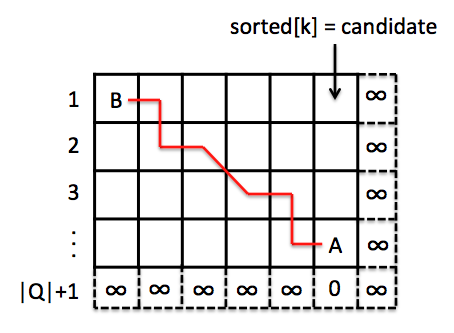
\includegraphics[scale=0.5]{dynamic_programming.png}
\end{center}
\caption{Dynamic Time Warping}
\end{figure}


The height represents the length of the query. Value A is initialized to 0, then computed as the minimum of the values on its right, bottom-right, the below sides, plus cost 1 if it moves horizontally or vertically. The values in the table are computed following this algorithm until it reaches the top-left of the table, which is the distance of the candidate. \par

\subsection{MapReduce}
Instead of a centralized algorithm (Algorithm 1), we propose here a distributed algorithm (Algorithm 2-4) via MapReduce. \par

\subsubsection*{Mappper}
For each input $(Q, X, \mathrm{candidate}, \mathrm{index})$, where $Q$ is the query, $X$ is the database sequence, \emph{candidate} is the candidate endpoint and \emph{index} is that of this candidate in the candidate array, we first compute the distance between the query and this candidate subsequence. We also compute the start point $j_{\mathrm{start}}$ and end point $j_{\mathrm{end}}$ of this matching. Afterwards, we associate it with a key, which is computed as $$\mathrm{key} = \mathrm{index}\ \%\ \mathrm{total\_nodes},$$ where \emph{total\_nodes} is the number of nodes in the cloud. According to the keys, we assign every candidate to its corresponding node, candidates $(Q, X, \mathrm{key}, \mathrm{distance}, j_{\mathrm{start}}, j_{\mathrm{end}})$ with the same key will be on the same node. \par

\begin{algorithm}
	\caption{Mapper}
	\begin{algorithmic}[1]
	\State $j$ = candidate + 1;
	\For{$i$ = $|Q|+1$ to 1}
		\State cost[$i$][$j$] = $\infty$;
	\EndFor
	\While{(true)}
		\State $j = j - 1$;
		\If{(candidate - $j \geq 2*|Q|)$}
			\State break;
		\EndIf
		\If{(candidate == $j$)}
			\State cost[$|Q|+1$][$j$] = 0;
			\State endpoint[$|Q|+1$][$j$] = $j$;
		\Else
			\State cost[$|Q|+1$][$j$] = $\infty$;
		\EndIf
		\For{$i$ = $|Q|$ to 1}
			\State previous = \{$(i+1, j), (i, j+1), (i+1, j+1)$\};
			\State $(p_i, p_j) = \mathrm{argmin}_{(a,b)\in\mathrm{previous}}\mathrm{cost}[a][b]$;
			\State cost$[i][j] = |Q_i - X_j| +$ cost$[p_i][p_j]$;
			\State endpoint$[i][j]$ = endpoint$[p_i][p_j]$;
		\EndFor
		\State $\mathrm{key} = \mathrm{index}\ \%\ \mathrm{total\_nodes}$;
		\State distance = cost[1][$j$];
		\State $j_{\mathrm{start}} = j$;
		\State $j_{\mathrm{end}} = \mathrm{endpoint}[1][j]$;
		\State Emit($Q$, $X$, key, distance, $j_{\mathrm{start}}$, $j_{\mathrm{end}}$);
	\EndWhile
	\end{algorithmic}
\end{algorithm}

\subsection*{Combiner}
Each combiner takes candidates on the same node and computes the smallest distance among the candidates on that node, then output the results to the reducer.\\
\textbf{input:} $(Q, X, \mathrm{key}, [(\mathrm{distance_1}, j_{\mathrm{start},1}, j_{\mathrm{end},1}),\ (\mathrm{distance_2}, j_{\mathrm{start},2}, j_{\mathrm{end},2}), \cdots])$ \\
\textbf{output:} $(Q, X, \mathrm{key}, \mathrm{distance_{min}}, j_{\mathrm{start}}, j_{\mathrm{end}})$ \par

\begin{algorithm}
	\caption{Combiner}
	\begin{algorithmic}[1]
		\State $\mathrm{distance_{min}} = \infty$;
		\ForAll{$\mathrm{distance_i}\in[\mathrm{distance_1}, \mathrm{distance_2}, \cdots]$}
			\If{($\mathrm{distance_i} < \mathrm{distance_{min}}$)}
				\State $\mathrm{distance_{min}} = \mathrm{distance_i}$;
				\State $j_{\mathrm{start}} = j_{\mathrm{start, i}}$;
				\State $j_{\mathrm{end}} = j_{\mathrm{end, i}}$;
			\EndIf
		\EndFor
		\State Emit($Q$, $X$, key, $\mathrm{distance_{min}}$, $j_{\mathrm{start}}$, $j_{\mathrm{end}}$);
	\end{algorithmic}
\end{algorithm}

\subsection*{Reducer}
The reducer takes inputs from combiners and computer the smallest distance among these inputs. The result contains the smallest distance of all the original candidates.\\
\textbf{input:} $(Q, X, [(\mathrm{key_1}, \mathrm{distance_1}, j_\mathrm{start, 1}, j_\mathrm{end, 1}),\ (\mathrm{key_2}, \mathrm{distance_2}, j_\mathrm{start, 2}, j_\mathrm{end, 2}),\ \cdots])$ \\
\textbf{output:} $(Q, X, \mathrm{key}, \mathrm{distance_{min}}, j_{\mathrm{start}}, j_{\mathrm{end}})$ \par

\begin{algorithm}
	\caption{Reducer}
	\begin{algorithmic}[1]
		\State $\mathrm{distance_{min}} = \infty$;
		\ForAll{$\mathrm{distance_i}\in[\mathrm{distance_1}, \mathrm{distance_2}, \cdots]$}
			\If{($\mathrm{distance_i} < \mathrm{distance_{min}}$)}
				\State key = $\mathrm{key_i}$;
				\State $\mathrm{distance_{min}} = \mathrm{distance_i}$;
				\State $j_{\mathrm{start}} = j_{\mathrm{start, i}}$;
				\State $j_{\mathrm{end}} = j_{\mathrm{end, i}}$;
			\EndIf
		\EndFor
		\State start = $j_{\mathrm{end}} - 3*|Q|$;
		\State end = $j_{\mathrm{end}} + |Q|$;
		\State Adjust $j_{\mathrm{start}}$ and $j_{\mathrm{end}}$ by running the DTW algorithm between $Q$ and $X^{\mathrm{start:end}}$;
	\end{algorithmic}
\end{algorithm}

\end{document}
